\chapter{Theoretical Background} \label{ch:background}

% \section{Quantum Chromodynamics}

% \section{Phase Transitions}

% \section{Quark-Gluon Plasma}

\section{Quantum Chromodynamics}\label{section:QCD}
%%%%%%%%%%%%%%%%%%%%%%%%%%%%%%%%%%%%%%%%%%%%%%%%%%%%%%%%%%%%%%%%%%%%%%%%%%%%%%%
The strong force is one of the four fundamental interactions in physics. At large scale, it is responsible for binding the nucleons together to give the nucleus its structure. At the smaller scale, it binds the fundamental units of subnuclear matter, the quarks, together to form the nucleons. The electrodynamic interaction between charged particles such as protons and electrons is described by quantum electrodynamics (QED) as mediated by photons; the strong interaction, albeit more complicated, is explained under the framework of quantum chromodynamics (QCD) as mediated by gluons. \cite{KAPUSTA1979461, Shuryak1988} ???? The quarks and gluons of QCD are collectively known as partons. The gluons are the gauge bosons of the Yang-Mills theory.

The Yang-Mills theory is a non-Abelian gauge theory. It has a Lagrangian that is described by several parameters, some of which are redundant and need to be gauged. This is done by a mathematical treatment as prescribed under a gauge theory. The gauge theory associated with the Yang-Mills theory is based on the SU(N) group. It is non-Abelian as represented by the transformations being non-commutative. QCD is a gauge theory that describes the application of the SU(3) symmetry transformations on the triplet of quarks, namely red, blue, and green, with the nomenclature having no physical dependence on the three primary colors. The Electroweak interaction, on the other hand, can be formalized under the gauge group SU(2)$\times$U(1). Together, they form the SU(3)$\times$SU(2)$\times$(U1) gauge theory called the standard model.
%Along with electric charge, mass and spin, quarks have the intrinsic property of color charge. 

One of the aspects in which QCD is different from QED is the confinement of partons. In QED, the fundamental particles are bound together by the Coulomb potential, which diminishes with distance between the charge-carrying particles, as demonstrated by the relation \ref{eqn:QED-potential}:
\begin{equation}\label{eqn:QED-potential}
V_{C}\propto\frac{1}{r} 
\end{equation}
where $V_{C}$ is the Coulomb potential, and $r$ is the spatial separation between the particles. This means that bound QED particles can be isolated by increasing their spatial separation. The QCD potential, on the other hand, has an extra linear term in it:
\begin{equation}\label{eqn:QCD-potential}
V_{QCD} = -\frac{4}{3}\frac{\alpha_{S}}{r} + {k}{r} 
\end{equation}
%(pg 7 https://www2.ph.ed.ac.uk/~muheim/teaching/np3/lect-qcd.pdf)
where $\alpha_{S}$ is the QCD fine-structure constant and $k$ is is the strengh of the color interaction ($~$1 GeV/fm). This means that the potential increases linearly with distance at large distances, and so an infinite amount of energy is required to separate quarks. Hence, we never observe isolated quarks and they are said to be confined, not just bound, to form composite structures called hadrons.\cite{0954-3899-32-3-R01} Composition of a quark and an anti-quark forms a meson and that of three quarks forms a baryon. In addition to having a color charge, a quark also carries a flavor. There are six different quarks based on the flavors they carry: up, down, top, bottom, beauty, and strange.

%QCD is a gauge theory. Its Lagrangian remains unchanged under certain transformations. The Lagrangian has a number of degrees of freedom, some of which are redundant and need to be gauged, meaning regulated by a particular mathematical treatment. That mathematical treatment, in which the transformations of the gauge group are non-commutative, is described by a non-Abelian gauge theory. The Yang-Mills theory is an example of it. In this theory, the gauge boson is the gluon. 
%These confined, bound states of quarks and gluons is color-neutral.
%, and it is ergonomically more favorable to create a quark-antiquark pair than to produce unbound quarks
%, and $\alpha\_{QED}$ is the coupling constant.

\section{Phase Transitions}
%%%%%%%%%%%%%%%%%%%%%%%%%%%%%%%%%%%%%%%%%%%%%%%%%%%%%%%%%%%%%%%%%%%%%%%%%%%%%%%%%%%%%%%%%%%%%%
In everyday life, we observe matter existing in four distinct phases: solid, liquid, gas, and plasma. Changes in physical conditions can lead to a transition from one of these phases to another, exemplified by the commonly observed coversion of ice to water. Distinctions among the various phases can be represented in a chart called the phase diagram.

The phase diagram consists of thermodynamic observables such as temperature and density on its axes. Curves in the phase diagram represent boundries of physical conditions at which two or more phases of matter can coexist in equilibrium. Crossing a boundary represents an abrupt transition from one phase to another; this abruptness is mathematically characterized by the discontinuity in the change of the derivative of the free energy -- a thermodynamic varible -- with respect to the physical quantities in the axes. There can also be regions in the diagram representing the ranges of physical conditions in which a smooth phase transition can take place.

One of the main focuses of current experimental and theoretical nuclear physics research is the study of the phase diagram of strongly interacting matter at a range of temperatures and baryon chemical potentials. In experiments involving the collisions of heavy ions at high and low energies, different regions of the phase diagram can be probed by varying the collision energy \cite{PhysRevC.93.024901}. For instance, the high-baryon chemical potential regime corresponds to lower beam energies and higher temperatures correspond to higher beam energies. The results of these experiments and model calculations can be used to study the nature of transitions in the QCD phase diagram.

A schematic representing the QCD phase diagram on the temperature (T) and quark chemical potential ($\mu$) plane is shown in Figure \ref{fig:PhaseDiagram} \cite{1742-6596-761-1-012066}. A second-order transition is predicted at low baryon chemical potentials (close to baryon-antibaryon symmetry) and high temperatures reminiscent of the early universe. Methods to study this region of the phase space will be explored in this thesis. At low temperatures and high chemical potentials, loose predictions have been made regarding the existence of exotic phases of high density matter, and programs, such as the Compressed Baryonic Matter experiment at the Facility for Antiproton and Ion Research in Germany, are being designed to study this region of the phase diagram.
% but within reach at modern facilities, specifically the Relativistic Heavy Ion Collider (RHIC) at the Brookhaven National Laboratory and the Large Hadron Collider (LHC) at CERN
%Details about these facilities are given in \ref{section:RHI-collisions}.
\begin{figure}[h]
  \centering
  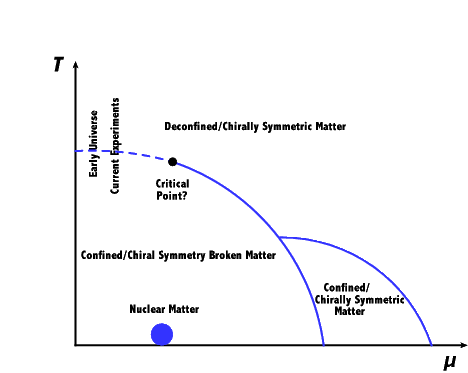
\includegraphics[width=5.5in]{figures/1742-6596-761-1-012066.png}\\
  \caption{Schematic of the QCD phase diagram \cite{1742-6596-761-1-012066}.}\label{fig:PhaseDiagram}
\end{figure}


\section{Quark-Gluon Plasma}
%%%%%%%%%%%%%%%%%%%%%%%%%%%%%%%%%%%%%%%%%%%%%%%%%%%%%%%%%%%%%%%%%%%%%%%%%%%%%%%%%%%%%%%%%%%%%%
The confinement of quarks into the hardonic phase of QCD matter, as described in section \ref{section:QCD}, has its limitations. At very high densities, when the wave function of a single hadron encompasses the spatial regions covered by multiple such hadrons, it is impossible to classify which pair or triplet of quarks belongs to which meson or baryon. As long as a particular quark is close enough to the other quarks in the volume, it is deconfined in such a way that it can freely move anywhere in the volume. \cite{0954-3899-32-3-R01} QCD predicts such phase transition, at energy densities above 0.2-1 GeV/fm$^{3}$ \cite{Adam:2139456} and around a critical temperature of about 200 MeV \cite{2013arXiv1304.1452M}, of strongly interacting matter to a phase with quarks and gluons in thermal and chemical equilibrium representing the relevant degrees of freedom and behaving like an almost perfect quantum fluid \cite{PhysRevLett.109.152303}. This deconfined state of quarks and gluons is termed the quark-gluon plasma (QGP) in analogy to the quantum electrodynamical plasma phase of matter.

%The deconfinement is what the weakening of the strong interaction due to the polarization of the QCD vacuum is expected to lead to at high energies. The expectation of this phase transition also makes sense in terms of the chiral symmetry of the QCD Lagrangian, which is spontaneously broken at low temperatures, but restored at high temperatures, providing a sufficient condition for the deconfinement.
% Existence of QGP in the early universe
% Production of QGP in the lab


